\section{Discussion}
\label{sec:discussion}

\subsection{Prevalence of Irish attacks}
\label{sec:irish_analysis}

Referring to section \ref{sec:origin_analysis}, it 
came as a rather large surprise that Ireland was the most 
common source of attackers. 

\begin{figure}[H]
    \centering
    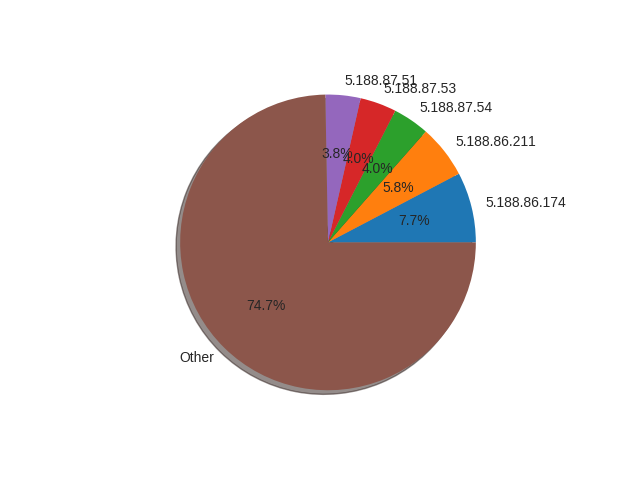
\includegraphics[width=0.8\textwidth]{src/images/ip_breakdown.png}
    \caption{Total attacks broken down by source address}
    \label{fig:attacks_by_ip}
\end{figure}


In fact, looking into the top offenders, 


\texttt{'5.188.86.174'},
\texttt{'5.188.86.211'},
\texttt{'5.188.87.53'},
\texttt{'5.188.87.54'}, and 
\texttt{'5.188.87.55'} 

reveals that all of them 
are owned by \texttt{'Petersburg 
Internet Network ltd.'}(PIN) which has been
implicated in both route-hijacking \cite{bogus_routing} 
and allegedly with a gang of cyber criminals \cite{petersburg}
